% Created 2021-09-11 Sat 17:16
% Intended LaTeX compiler: pdflatex
\documentclass{scrartcl}
\usepackage[utf8]{inputenc}
\usepackage[T1]{fontenc}
\usepackage{fontspec}
\usepackage{graphicx}
\usepackage{grffile}
\usepackage{longtable}
\usepackage{wrapfig}
\usepackage{rotating}
\usepackage[normalem]{ulem}
\usepackage{amsmath}
\usepackage{textcomp}
\usepackage{amssymb}
\usepackage{capt-of}
\usepackage[dvipsnames]{xcolor}
\usepackage[colorlinks=true, linkcolor=Blue, citecolor=BrickRed, urlcolor=PineGreen]{hyperref}
\usepackage{indentfirst}
\setmainfont[Ligatures=TeX]{Alegreya}
\setmonofont[Ligatures=TeX]{Liga SFMono Nerd Font}
% features: (acronym underline par-sep engraved-code-setup engraved-code)
\newcommand{\acr}[1]{\protect\textls*[110]{\scshape #1}}
\newcommand{\acrs}{\protect\scalebox{.91}[.84]\hspace{0.15ex}s}
\usepackage[normalem]{ulem}
\setlength{\parskip}{\baselineskip}
\setlength{\parindent}{0pt}


\usepackage{fvextra}
\fvset{
  commandchars=\\\{\},
  highlightcolor=white!95!black!80!blue,
  breaklines=true,
  breaksymbol=\color{white!60!black}\tiny\ensuremath{\hookrightarrow}}
\renewcommand\theFancyVerbLine{\footnotesize\color{black!40!white}\arabic{FancyVerbLine}}

\definecolor{codebackground}{HTML}{f7f7f7}
\definecolor{codeborder}{HTML}{f0f0f0}

% TODO have code boxes keep line vertical alignment
\usepackage[breakable,xparse]{tcolorbox}
\DeclareTColorBox[]{Code}{o}%
{colback=codebackground, colframe=codeborder,
  fontupper=\footnotesize,
  colupper=EFD,
  IfNoValueTF={#1}%
  {boxsep=2pt, arc=2.5pt, outer arc=2.5pt,
    boxrule=0.5pt, left=2pt}%
  {boxsep=2.5pt, arc=0pt, outer arc=0pt,
    boxrule=0pt, leftrule=1.5pt, left=0.5pt},
  right=2pt, top=1pt, bottom=0.5pt,
  breakable}

\definecolor{EFD}{HTML}{383a42}
\newcommand{\EFD}[1]{\textcolor{EFD}{#1}} % default
\definecolor{EFk}{HTML}{e45649}
\newcommand{\EFk}[1]{\textcolor{EFk}{#1}} % font-lock-keyword-face
\definecolor{EFd}{HTML}{84888b}
\newcommand{\EFd}[1]{\textcolor{EFd}{\textit{#1}}} % font-lock-doc-face
\definecolor{EFt}{HTML}{986801}
\newcommand{\EFt}[1]{\textcolor{EFt}{#1}} % font-lock-type-face
\definecolor{EFs}{HTML}{50a14f}
\newcommand{\EFs}[1]{\textcolor{EFs}{#1}} % font-lock-string-face
\definecolor{EFw}{HTML}{986801}
\newcommand{\EFw}[1]{\textcolor{EFw}{#1}} % font-lock-warning-face
\definecolor{EFb}{HTML}{a626a4}
\newcommand{\EFb}[1]{\textcolor{EFb}{#1}} % font-lock-builtin-face
\definecolor{EFct}{HTML}{9ca0a4}
\newcommand{\EFct}[1]{\textcolor{EFct}{#1}} % font-lock-comment-face
\definecolor{EFc}{HTML}{b751b6}
\newcommand{\EFc}[1]{\textcolor{EFc}{#1}} % font-lock-constant-face
\definecolor{EFpp}{HTML}{4078f2}
\newcommand{\EFpp}[1]{\textcolor{EFpp}{\textbf{#1}}} % font-lock-preprocessor-face
\definecolor{EFnc}{HTML}{4078f2}
\newcommand{\EFnc}[1]{\textcolor{EFnc}{\textbf{#1}}} % font-lock-negation-char-face
\definecolor{EFv}{HTML}{6a1868}
\newcommand{\EFv}[1]{\textcolor{EFv}{#1}} % font-lock-variable-name-face
\definecolor{EFf}{HTML}{a626a4}
\newcommand{\EFf}[1]{\textcolor{EFf}{#1}} % font-lock-function-name-face
\definecolor{EFcd}{HTML}{9ca0a4}
\newcommand{\EFcd}[1]{\textcolor{EFcd}{#1}} % font-lock-comment-delimiter-face
\definecolor{EFrc}{HTML}{4078f2}
\newcommand{\EFrc}[1]{\textcolor{EFrc}{\textbf{#1}}} % font-lock-regexp-grouping-construct
\definecolor{EFrb}{HTML}{4078f2}
\newcommand{\EFrb}[1]{\textcolor{EFrb}{\textbf{#1}}} % font-lock-regexp-grouping-backslash
\newcommand{\EFob}[1]{#1} % org-block
\definecolor{EFhn}{HTML}{da8548}
\newcommand{\EFhn}[1]{\textcolor{EFhn}{\textbf{#1}}} % highlight-numbers-number
\definecolor{EFhq}{HTML}{4078f2}
\newcommand{\EFhq}[1]{\textcolor{EFhq}{#1}} % highlight-quoted-quote
\definecolor{EFhs}{HTML}{986801}
\newcommand{\EFhs}[1]{\textcolor{EFhs}{#1}} % highlight-quoted-symbol
\definecolor{EFrdi}{HTML}{4078f2}
\newcommand{\EFrdi}[1]{\textcolor{EFrdi}{#1}} % rainbow-delimiters-depth-1-face
\definecolor{EFrdii}{HTML}{a626a4}
\newcommand{\EFrdii}[1]{\textcolor{EFrdii}{#1}} % rainbow-delimiters-depth-2-face
\definecolor{EFrdiii}{HTML}{50a14f}
\newcommand{\EFrdiii}[1]{\textcolor{EFrdiii}{#1}} % rainbow-delimiters-depth-3-face
\definecolor{EFrdiv}{HTML}{da8548}
\newcommand{\EFrdiv}[1]{\textcolor{EFrdiv}{#1}} % rainbow-delimiters-depth-4-face
\definecolor{EFrdv}{HTML}{b751b6}
\newcommand{\EFrdv}[1]{\textcolor{EFrdv}{#1}} % rainbow-delimiters-depth-5-face
\definecolor{EFrdvi}{HTML}{986801}
\newcommand{\EFrdvi}[1]{\textcolor{EFrdvi}{#1}} % rainbow-delimiters-depth-6-face
\definecolor{EFrdvii}{HTML}{4db5bd}
\newcommand{\EFrdvii}[1]{\textcolor{EFrdvii}{#1}} % rainbow-delimiters-depth-7-face
\definecolor{EFrdiix}{HTML}{80a880}
\newcommand{\EFrdiix}[1]{\textcolor{EFrdiix}{#1}} % rainbow-delimiters-depth-8-face
\definecolor{EFrdix}{HTML}{887070}
\newcommand{\EFrdix}[1]{\textcolor{EFrdix}{#1}} % rainbow-delimiters-depth-9-face
% end features

%% make document follow Emacs theme

\definecolor{obg}{HTML}{242730}
\definecolor{ofg}{HTML}{bbc2cf}

\pagecolor{obg}
\color{ofg}

% list labels

\definecolor{itemlabel}{HTML}{51afef}

\renewcommand{\labelitemi}{\textcolor{itemlabel}{\textbullet}}
\renewcommand{\labelitemii}{\textcolor{itemlabel}{\normalfont\bfseries \textendash}}
\renewcommand{\labelitemiii}{\textcolor{itemlabel}{\textasteriskcentered}}
\renewcommand{\labelitemiv}{\textcolor{itemlabel}{\textperiodcentered}}

\renewcommand{\labelenumi}{\textcolor{itemlabel}{\theenumi.}}
\renewcommand{\labelenumii}{\textcolor{itemlabel}{(\theenumii)}}
\renewcommand{\labelenumiii}{\textcolor{itemlabel}{\theenumiii.}}
\renewcommand{\labelenumiv}{\textcolor{itemlabel}{\theenumiv.}}

% structural elements

\definecolor{documentTitle}{HTML}{C57BDB}
\definecolor{documentInfo}{HTML}{C57BDB}
\definecolor{level1}{HTML}{51afef}
\definecolor{level2}{HTML}{C57BDB}
\definecolor{level3}{HTML}{a991f1}
\definecolor{level4}{HTML}{7cc3f3}
\definecolor{level5}{HTML}{d39ce3}
\definecolor{level6}{HTML}{a8d7f7}
\definecolor{level7}{HTML}{e2bded}
\definecolor{level8}{HTML}{dceffb}

\addtokomafont{title}{\color{documentTitle}}
\addtokomafont{author}{\color{documentInfo}}
\addtokomafont{date}{\color{documentInfo}}
\addtokomafont{section}{\color{level1}}
\newkomafont{sectionprefix}{\color{level1}}
\addtokomafont{subsection}{\color{level2}}
\newkomafont{subsectionprefix}{\color{level2}}
\addtokomafont{subsubsection}{\color{level3}}
\newkomafont{subsubsectionprefix}{\color{level3}}
\addtokomafont{paragraph}{\color{level4}}
\newkomafont{paragraphprefix}{\color{level4}}
\addtokomafont{subparagraph}{\color{level5}}
\newkomafont{subparagraphprefix}{\color{level5}}

% textual elements

\definecolor{link}{HTML}{51afef}
\definecolor{cite}{HTML}{800080}
\definecolor{itemlabel}{HTML}{51afef}
\definecolor{code}{HTML}{e69055}
\definecolor{verbatim}{HTML}{7bc275}

\renewcommand{\labelitemi}{\textcolor{itemlabel}{\textbullet}}
\renewcommand{\labelitemii}{\textcolor{itemlabel}{\normalfont\bfseries \textendash}}
\renewcommand{\labelitemiii}{\textcolor{itemlabel}{\textasteriskcentered}}
\renewcommand{\labelitemiv}{\textcolor{itemlabel}{\textperiodcentered}}

\renewcommand{\labelenumi}{\textcolor{itemlabel}{\theenumi.}}
\renewcommand{\labelenumii}{\textcolor{itemlabel}{(\theenumii)}}
\renewcommand{\labelenumiii}{\textcolor{itemlabel}{\theenumiii.}}
\renewcommand{\labelenumiv}{\textcolor{itemlabel}{\theenumiv.}}

\DeclareTextFontCommand{\texttt}{\color{code}\ttfamily}
\makeatletter
\def\verbatim@font{\color{verbatim}\normalfont\ttfamily}
\makeatother

% code blocks

\definecolor{codebackground}{HTML}{272a33}
\colorlet{EFD}{ofg}
\definecolor{codeborder}{HTML}{2b2e37}

%% end customisations

\author{Shaurya Singh}
\date{\today}
\title{Password Generating Algorithm (Assignment \#1)}
\colorlet{greenyblue}{blue!70!green}
\colorlet{blueygreen}{blue!40!green}
\providecolor{link}{named}{greenyblue}
\providecolor{cite}{named}{blueygreen}
\hypersetup{
  pdfauthor={Shaurya Singh},
  pdftitle={Password Generating Algorithm (Assignment \#1)},
  pdfkeywords={},
  pdfsubject={},
  pdfcreator={Emacs 28.0.50 (Org mode 9.5)},
  pdflang={English},
  breaklinks=true,
  colorlinks=true,
  linkcolor=,
  urlcolor=link,
  citecolor=cite
}
\urlstyle{same}
\begin{document}

\maketitle
\setcounter{tocdepth}{2}
\tableofcontents

\begin{center}
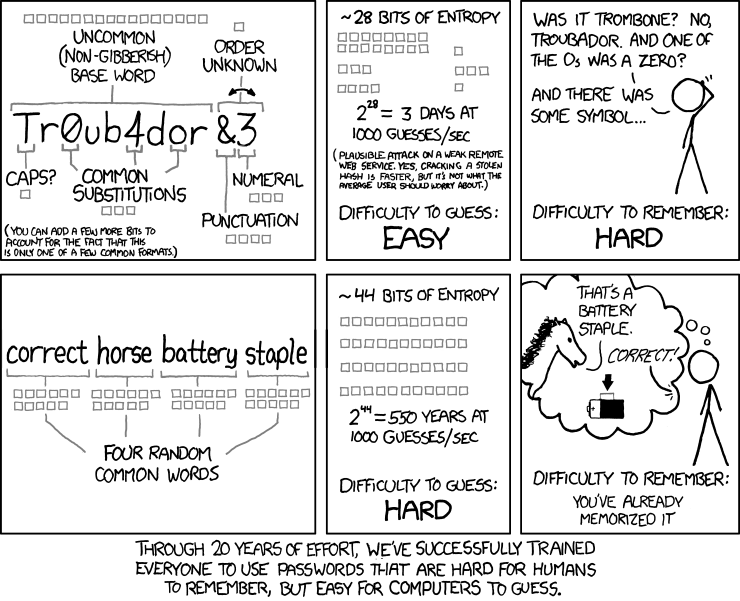
\includegraphics[width=.9\linewidth]{./password_strength_xkcd.png}
\end{center}

\section{Entropy and Creating Passwords}
\label{sec:org8cecec5}
\subsection{What is Entropy?}
\label{sec:org84fc06e}
Entropy is a measure of ``uncertainty'' in an outcome. In this context, it can be
thought of as a value representing how unpredictable the next character of of a
password is. It is calculated as \(\log_{2}(a^{b})\) where a is the number of allowed
symbols and b is its length.

\subsection{Why \texttt{Tr0ub4dor\&3} is a Bad Password}
\label{sec:orgb6c5b1e}
A truly random string of length 11 (not like ``Tr0ub4dor\&3'', but more like
``J4I/tyJ\&Acy'') has \(\log_{2}(94^{11})=72.1\) bits, with \(94\) being the total number of
letters, numbers, and symbols one can choose. However the comic shows that
``Tr0ub4dor\&3'' has only \(28\) bits of entropy. This is because the password follows
a simple pattern of a dictionary word + a couple extra numbers or symbols, hence
the entropy calculation is more appropriately expressed with \(\log_{2}(65000\times94\times94)\)
with \(65000\) representing a rough estimate of all dictionary words people are
likely to choose.

\subsection{Creating High-Entropy Passwords You Can Remember}
\label{sec:orga55b5e6}
Another way of selecting a password is to have \(2048\) ``symbols'' (common words) and
select only \(4\) of those symbols. \(\log_{2}(2048^{4})=44\) bits, much better than \(28\).

It is absolutely true that people make passwords hard to remember because they
think they are ``safer'', and it is certainly true that length, all other things
being equal, tends to make for very strong passwords So, Instead of creating a
randomly generated string of letters (which is what a random password generator
would do), it makes sense to link together common word. This offers similar
entropy levels, while being much easier to remember

\section{The Algorithm}
\label{sec:org76d54f1}
\subsection{Our algorithm is going to}
\label{sec:orga6ec109}
\begin{enumerate}
\item Take an input (number of words in the password (\texttt{nwords}) + numbers of bits per
word (\texttt{nbits}))
\item Read a wordlist file, which contains 45k words along with their frequency
\item Pick \texttt{nwords} words
\item Join those words together
\item Print the password
\item Calculate entropy for the password
\item Calculate/print what \#bit key the password is equal to
\item Calculate/print how many years it will take to crack the password (with cpu,
then with gpu)
\end{enumerate}

\subsection{Formulas used to calculate}
\label{sec:orgc173721}
Calculating entropy:
\(\text{entropy}=\text{number of bits}\times\text{number of words}\)

Calculating years need to crack code
\(\text{years}=\text{entropy}/\text{crypts per second}/\text{seconds in a day}/\text{days in a year}\)
\(\text{entropy}/\text{crypts per second}/86400/365\)

\subsection{Sample:}
\label{sec:org2858264}
The following example runs the program, telling it to create a 5 word password.
Since the wordlist we use has varied word legnths, we can't calculate entropy
the conventional way. However, the author has estimated the list has 11 bits per
word, so the program assumes 11 bits/word by default
\begin{Code}
\begin{Verbatim}[]
\color{EFD}\char126{}/o/csp/assignment1 [master] λ python3 algorithm.py \EFhn{5}

Your password is \EFs{"strike ready thought these find"}.
That\EFs{'s equivalent to a 55-bit key.

That password would take 1.6e+02 years to crack
on my core 2 duo from 2009, assuming an attack on a MS-Cache hash,
(the worst password hashing algorithm in common use)

The most common password-hashing algorithm is md5, cracking such a hash would take 3.2e+05 years.

But a modern GPU can crack about 250 times as fast,
so that same iterated MD5 would fall in 1.3e+03 years.}
\end{Verbatim}
\end{Code}

\subsection{Code}
\label{sec:org992182f}
The python code used to calculate this is below
\begin{Code}
\begin{Verbatim}[]
\color{EFD}\textcolor[HTML]{9ca0a4}{\#!/usr/bin/env python3}
\textcolor[HTML]{9ca0a4}{\# Insipred by http://xkcd.com/936/}

\textcolor[HTML]{9ca0a4}{\# Import what we need}
\textcolor[HTML]{e45649}{import} random, itertools, os, sys

\textcolor[HTML]{e45649}{def} \textcolor[HTML]{a626a4}{main}(\textcolor[HTML]{6a1868}{argv}):
    \textcolor[HTML]{9ca0a4}{\# number of words should be first input from the program}
    \textcolor[HTML]{e45649}{try}:
        nwords \textcolor[HTML]{e45649}{=} \textcolor[HTML]{a626a4}{\textbf{int}}(argv[\textcolor[HTML]{b751b6}{1}])
    \textcolor[HTML]{e45649}{except} \textcolor[HTML]{986801}{IndexError}:
        \textcolor[HTML]{e45649}{return} \textcolor[HTML]{51afef}{\textbf{usage}}(argv[\textcolor[HTML]{b751b6}{0}])

    \textcolor[HTML]{9ca0a4}{\# number of bits should be second input from the program}
    \textcolor[HTML]{e45649}{try}:
        nbits \textcolor[HTML]{e45649}{=} \textcolor[HTML]{a626a4}{\textbf{int}}(argv[\textcolor[HTML]{b751b6}{2}])
    \textcolor[HTML]{e45649}{except} \textcolor[HTML]{986801}{IndexError}:
        nbits \textcolor[HTML]{e45649}{=} \textcolor[HTML]{b751b6}{11}

    \textcolor[HTML]{9ca0a4}{\# read the wordlist}
    \EFv{filename} \textcolor[HTML]{e45649}{=} os.\textcolor[HTML]{b751b6}{\textit{path}}.\textcolor[HTML]{51afef}{\textbf{\textit{join}}}(os.\textcolor[HTML]{b751b6}{\textit{environ}}[\textcolor[HTML]{50a14f}{'HOME'}], \textcolor[HTML]{50a14f}{'org'}, \textcolor[HTML]{50a14f}{'csp'}, \textcolor[HTML]{50a14f}{'assignment1'}, \textcolor[HTML]{50a14f}{'wordlist'})
    \EFv{wordlist} \textcolor[HTML]{e45649}{=} \textcolor[HTML]{51afef}{\textbf{read\_file}}(filename, nbits)
    \textcolor[HTML]{e45649}{if} \textcolor[HTML]{a626a4}{\textbf{len}}(wordlist) \textcolor[HTML]{e45649}{!=} \textcolor[HTML]{b751b6}{2}\textcolor[HTML]{e45649}{**}nbits:
        sys.\textcolor[HTML]{b751b6}{\textit{stderr}}.\textcolor[HTML]{51afef}{\textbf{\textit{write}}}(\textcolor[HTML]{50a14f}{"\%r contains only \%d words, not \%d.}\textcolor[HTML]{e45649}{\char92{}n}\textcolor[HTML]{50a14f}{"} \textcolor[HTML]{e45649}{\%}
                         (filename, \textcolor[HTML]{a626a4}{\textbf{len}}(wordlist), \textcolor[HTML]{b751b6}{2}\textcolor[HTML]{e45649}{**}nbits))
        \textcolor[HTML]{e45649}{return} \textcolor[HTML]{b751b6}{2}

    \textcolor[HTML]{9ca0a4}{\# generate the password, then display it}
    \textcolor[HTML]{51afef}{\textbf{display\_password}}(\textcolor[HTML]{51afef}{\textbf{generate\_password}}(nwords, wordlist), nwords, nbits)
    \textcolor[HTML]{e45649}{return} \textcolor[HTML]{b751b6}{0}

\textcolor[HTML]{9ca0a4}{\# Info about the usage of the program, if the user gives an incorrect input}
\textcolor[HTML]{e45649}{def} \textcolor[HTML]{a626a4}{usage}(\textcolor[HTML]{6a1868}{argv0}):
    \EFv{p} \textcolor[HTML]{e45649}{=} sys.\textcolor[HTML]{b751b6}{\textit{stderr}}.\textcolor[HTML]{b751b6}{\textit{write}}
    \textcolor[HTML]{51afef}{\textbf{p}}(\textcolor[HTML]{50a14f}{"Usage: \%s nwords [nbits]}\textcolor[HTML]{e45649}{\char92{}n}\textcolor[HTML]{50a14f}{"} \textcolor[HTML]{e45649}{\%} argv0)
    \textcolor[HTML]{51afef}{\textbf{p}}(\textcolor[HTML]{50a14f}{"Generates a password of nwords words, each with nbits bits}\textcolor[HTML]{e45649}{\char92{}n}\textcolor[HTML]{50a14f}{"})
    \textcolor[HTML]{51afef}{\textbf{p}}(\textcolor[HTML]{50a14f}{"of entropy, choosing words from the first entries in}\textcolor[HTML]{e45649}{\char92{}n}\textcolor[HTML]{50a14f}{"})
    \textcolor[HTML]{51afef}{\textbf{p}}(\textcolor[HTML]{50a14f}{"<http://canonical.org/\char126{}kragen/sw/wordlist>, which is a text file}\textcolor[HTML]{e45649}{\char92{}n}\textcolor[HTML]{50a14f}{"})
    \textcolor[HTML]{51afef}{\textbf{p}}(\textcolor[HTML]{50a14f}{"with one word per line, preceded by its frequency, most frequent}\textcolor[HTML]{e45649}{\char92{}n}\textcolor[HTML]{50a14f}{"})
    \textcolor[HTML]{51afef}{\textbf{p}}(\textcolor[HTML]{50a14f}{"words first.}\textcolor[HTML]{e45649}{\char92{}n}\textcolor[HTML]{50a14f}{"})
    \textcolor[HTML]{51afef}{\textbf{p}}(\textcolor[HTML]{50a14f}{"}\textcolor[HTML]{e45649}{\char92{}n}\textcolor[HTML]{50a14f}{Recommended:}\textcolor[HTML]{e45649}{\char92{}n}\textcolor[HTML]{50a14f}{"})
    \textcolor[HTML]{51afef}{\textbf{p}}(\textcolor[HTML]{50a14f}{"    \%s 5 12}\textcolor[HTML]{e45649}{\char92{}n}\textcolor[HTML]{50a14f}{"} \textcolor[HTML]{e45649}{\%} argv0)
    \textcolor[HTML]{51afef}{\textbf{p}}(\textcolor[HTML]{50a14f}{"    \%s 6}\textcolor[HTML]{e45649}{\char92{}n}\textcolor[HTML]{50a14f}{"} \textcolor[HTML]{e45649}{\%} argv0)
    \textcolor[HTML]{e45649}{return} \textcolor[HTML]{b751b6}{1}

\textcolor[HTML]{9ca0a4}{\# function to read the wordlist file}
\textcolor[HTML]{e45649}{def} \textcolor[HTML]{a626a4}{read\_file}(\textcolor[HTML]{6a1868}{filename}, \textcolor[HTML]{6a1868}{nbits}):
    \textcolor[HTML]{e45649}{return} [line.\textcolor[HTML]{51afef}{\textbf{\textit{split}}}()[\textcolor[HTML]{b751b6}{1}] \textcolor[HTML]{e45649}{for} \textcolor[HTML]{6a1868}{line} \textcolor[HTML]{e45649}{in}
            itertools.\textcolor[HTML]{51afef}{\textbf{\textit{islice}}}(\textcolor[HTML]{a626a4}{\textbf{open}}(filename), \textcolor[HTML]{b751b6}{2}\textcolor[HTML]{e45649}{**}nbits)]

\textcolor[HTML]{9ca0a4}{\# function to generate the password (random words from wordlist)}
\textcolor[HTML]{e45649}{def} \textcolor[HTML]{a626a4}{generate\_password}(\textcolor[HTML]{6a1868}{nwords}, \textcolor[HTML]{6a1868}{wordlist}):
    \EFv{choice} \textcolor[HTML]{e45649}{=} random.\textcolor[HTML]{986801}{\textbf{\textit{SystemRandom}}}().\textcolor[HTML]{b751b6}{\textit{choice}}
    \textcolor[HTML]{e45649}{return} \textcolor[HTML]{50a14f}{' '}.\textcolor[HTML]{51afef}{\textbf{\textit{join}}}(\textcolor[HTML]{51afef}{\textbf{choice}}(wordlist) \textcolor[HTML]{e45649}{for} \textcolor[HTML]{6a1868}{ii} \textcolor[HTML]{e45649}{in} \textcolor[HTML]{a626a4}{\textbf{range}}(nwords))

\textcolor[HTML]{9ca0a4}{\# function to display info about the password}
\textcolor[HTML]{e45649}{def} \textcolor[HTML]{a626a4}{display\_password}(\textcolor[HTML]{6a1868}{password}, \textcolor[HTML]{6a1868}{nwords}, \textcolor[HTML]{6a1868}{nbits}):
    \textcolor[HTML]{a626a4}{\textbf{print}}(\textcolor[HTML]{50a14f}{'Your password is "\%s".'} \textcolor[HTML]{e45649}{\%} password)

    \textcolor[HTML]{9ca0a4}{\# entropy value is equal the the number of words * the number of bits in each word}
    \EFv{entropy} \textcolor[HTML]{e45649}{=} nwords \textcolor[HTML]{e45649}{*} nbits
    \textcolor[HTML]{a626a4}{\textbf{print}}(\textcolor[HTML]{50a14f}{"That's equivalent to a \%d-bit key."} \textcolor[HTML]{e45649}{\%} entropy)
    \textcolor[HTML]{a626a4}{\textbf{print}}()

    \textcolor[HTML]{9ca0a4}{\# john --test (<http://www.openwall.com/john/>) reports that it}
    \textcolor[HTML]{9ca0a4}{\# can do 7303000 MD5 operations per second, but I’m pretty sure}
    \textcolor[HTML]{9ca0a4}{\# that’s a single-core number}
    \EFv{t} \textcolor[HTML]{e45649}{=} \textcolor[HTML]{51afef}{\textbf{years}}(entropy, \textcolor[HTML]{b751b6}{7303000})
    \textcolor[HTML]{a626a4}{\textbf{print}}(\textcolor[HTML]{50a14f}{"That password would take \%.2g years to crack"} \textcolor[HTML]{e45649}{\%} t)
    \textcolor[HTML]{a626a4}{\textbf{print}}(\textcolor[HTML]{50a14f}{"on my core 2 duo from 2009, assuming an attack on a MS-Cache hash,"})
    \textcolor[HTML]{a626a4}{\textbf{print}}(\textcolor[HTML]{50a14f}{"(the worst password hashing algorithm in common use)"})
    \textcolor[HTML]{a626a4}{\textbf{print}}()

    \EFv{t} \textcolor[HTML]{e45649}{=} \textcolor[HTML]{51afef}{\textbf{years}}(entropy, \textcolor[HTML]{b751b6}{3539})
    \textcolor[HTML]{a626a4}{\textbf{print}}(\textcolor[HTML]{50a14f}{"The most common password-hashing algorithm is md5, cracking such a hash would take \%.2g years."} \textcolor[HTML]{e45649}{\%} t)
    \textcolor[HTML]{a626a4}{\textbf{print}}()

    \textcolor[HTML]{9ca0a4}{\# <https://en.bitcoin.it/wiki/Mining\_hardware\_comparison> says a}
    \textcolor[HTML]{9ca0a4}{\# The same mining-hardware comparison says a Radeon 5870 card can}
    \textcolor[HTML]{9ca0a4}{\# do 393.46 Mhash/s for US\$350.}
    \textcolor[HTML]{a626a4}{\textbf{print}}(\textcolor[HTML]{50a14f}{"But a modern GPU can crack about 250 times as fast,"})
    \textcolor[HTML]{a626a4}{\textbf{print}}(\textcolor[HTML]{50a14f}{"so that same iterated MD5 would fall in \%.2g years."} \textcolor[HTML]{e45649}{\%} (t \textcolor[HTML]{e45649}{/} \textcolor[HTML]{b751b6}{250}))
    \textcolor[HTML]{a626a4}{\textbf{print}}()

\textcolor[HTML]{9ca0a4}{\# function to calculate years of entropy}
\textcolor[HTML]{e45649}{def} \textcolor[HTML]{a626a4}{years}(\textcolor[HTML]{6a1868}{entropy}, \textcolor[HTML]{6a1868}{crypts\_per\_second}):
    \textcolor[HTML]{9ca0a4}{\# entropy divided by crypts/s for inputed hash, divided by seconds/day, divided by days/year}
    \textcolor[HTML]{e45649}{return} \textcolor[HTML]{a626a4}{\textbf{float}}(\textcolor[HTML]{b751b6}{2}\textcolor[HTML]{e45649}{**}entropy) \textcolor[HTML]{e45649}{/} crypts\_per\_second \textcolor[HTML]{e45649}{/} \textcolor[HTML]{b751b6}{86400} \textcolor[HTML]{e45649}{/} \textcolor[HTML]{b751b6}{365}

\textcolor[HTML]{e45649}{if} \textcolor[HTML]{a626a4}{\_\_name\_\_} \textcolor[HTML]{e45649}{==} \textcolor[HTML]{50a14f}{'\_\_main\_\_'}:
    sys.\textcolor[HTML]{51afef}{\textbf{\textit{exit}}}(\textcolor[HTML]{51afef}{\textbf{main}}(sys.\textcolor[HTML]{b751b6}{\textit{argv}}))

\end{Verbatim}
\end{Code}
\end{document}
